\documentclass[a5paper,12pt]{article}
\usepackage{../../style}


\newcommand{\montitre}{Fiche C }


\begin{document}

\fiche{C : Variables numériques}
\titre{Variables et affichage} \\
\begin{tabular}{lllcc}
 & & printf & scanf (&) \\
(unsigned) & char & \%c & \%c \\
(const) & int & \%d & \%d \\
 & long & \%ld & \%ld \\
 & float & \%f & \%f \\
 & double & \%f & \%lf \\
\end{tabular}

\par

\titre{Opérateurs} \\ $+ \; ; \; - \; ; \; * \; ; \; / \; ; \; \% \; ; \; ++ \; ; \; -- \; ; \; += \; ; \; -= \; ; \; *= \; ; \; /= \; ; \; \%=$

\par

\titre{math.h}
\begin{itemize}
	\item fabs
	\item ceil
	\item floor
	\item pow
	\item sqrt
	\item sin, cos, tan
	\item asin, acos, atan
	\item exp, log, log10
\end{itemize}

\titre{Aléatoire : } srand(time(NULL)) puis rand()\%k



\fiche{C : Booléens et conditions}
\titre{Opérateurs} : $== \; ; \; > \; ; \; < \; ; \; >= \; ; \; <= \; ; \; != \; ; \; \&\& \; ; \; || \; ; \; !$

\par

\titre{Valeurs booléennes} 
\begin{itemize}
	\item 0 = faux
	\item 1 ou autre valeur = vrai
\end{itemize}

\par

\titre{Condition} \\
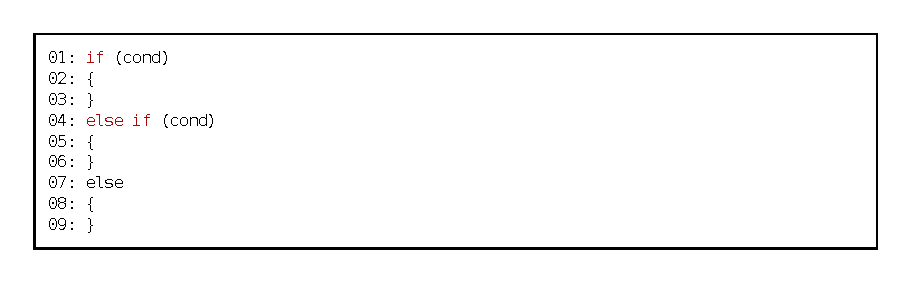
\includegraphics[width=\linewidth]{D6_1.pdf}

\par

\titre{Switch} \\
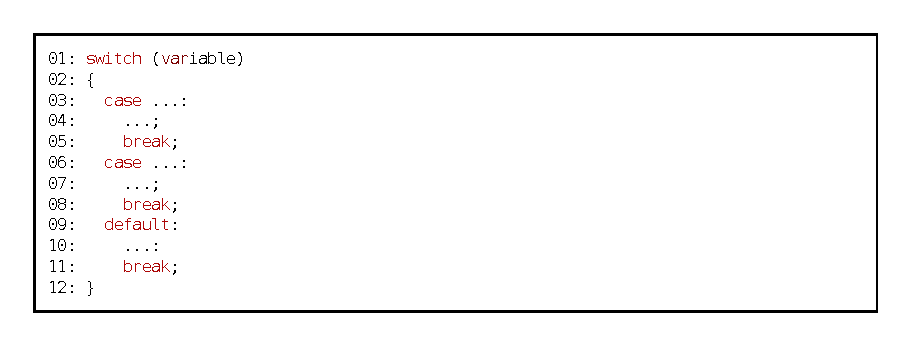
\includegraphics[width=\linewidth]{D6_2.pdf}

\par

\titre{Ternaire} \\
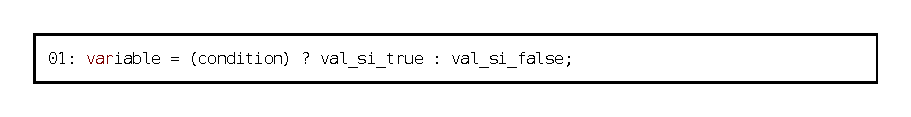
\includegraphics[width=\linewidth]{D6_3.pdf}

\vspace{-0.5cm}


\fiche{C : Boucles}

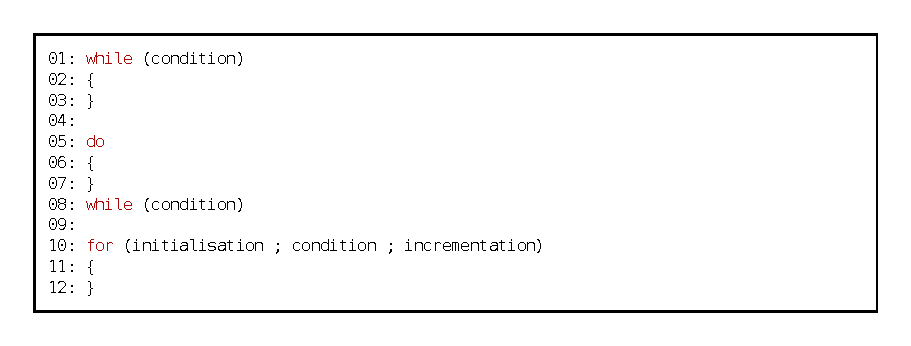
\includegraphics[width=\linewidth]{D7_1.pdf}



\fiche{C : fonctions}

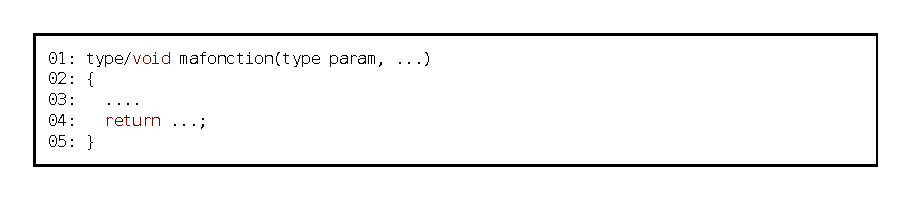
\includegraphics[width=\linewidth]{D8_1.pdf}

\par

\titre{Prototype}
Au début du fichier juste après les instructions pré-processeur \\
Ou dans un fichier header.h

\par

\titre{Portée des variables}
\begin{itemize}
\item Dans une fonction : locale
\item Dans une fonction + static : locale mais la valeur est conservé entre chaque appel
\item En dehors d'une fonction : globale (tout le programme)
\item En dehors d'une fonction + static : tout le fichier
\end{itemize}

\titre{Portée d'une fonction}
\begin{itemize}
\item En général : globale (tout le programme)
\item + static : tout le fichier
\end{itemize} 


\fiche{C : Pointeurs}
\titre{Afficher l'adresse d'une variable} : printf("\%p",\&mavariable) \\

\par

\titre{Créer un pointeur} (variable contenant l'adresse d'une autre variable) \\
type *monpointeur = NULL; \\
monpointeur = \&mavariable; \\

\par
\titre{Accéder à une variable via un pointeur} \\
printf("\%d",monpointeur) -> adresse de mavariable \\
printf("\%d",*monpointeur) -> valeur de mavariable \\

\par
\titre{Cas d'utilisation} \\
Envoyer un pointeur à une fonction permet de l'autoriser à modifier ponctuellement la valeur d'une variable sans pour autant la rendre globale. On envoie à la fonction l'adresse d'une variable à modifier à cet instant t.\\

\par

\titre{Différences tableau/pointeur :} Un tableau est un pointeur constant (on ne peut pas changer l'adresse pointée par un tableau. \\

\par

\titre{Type void* : } En général, on donne un type au pointeur pour connaître la "taille" d'une case en mémoire (en fait pointeur = adresse + taille). Avec un type void*, le type n'est pas imposé mais l'indirection est impossible sans typecast.

\newpage
\titre{exemple : memcopy}


\fiche{C : Mémoire}
\titre{La pile d'éxécution :} Elle contient les variables locales aux fonctions. Les fonctions s'empilent les unes sur les autres avec à la base la fonction main.\\

\par

\titre{Le segment de données :} Il contient les variables globales ou déclarées static. \\

\par

\titre{Le tas :} Il contient les variables allouées dynamiquement (malloc, calloc, realloc). La mémoire doit aussi être libérée dynamiquement avec free.\\

\par

\titre{Exemple}
\newpage


\fiche{C : Pointeurs de fonction}
\titre{Nom d'une fonction :} Le nom d'une fonction correspond à l'adresse du code source binaire de la fonction + sa signature (type de retour + types des paramètres).\\

\par

\titre{Définir un type pointeur de fonction :} typedef TypeRetour (*NomTypePtrFonc) (TypeParam1, TypeParam2 ... ) \\

\par

\titre{Exemple :}



\fiche{C : POO}
\titre{Exemples :}


\end{document}
